\documentclass{article}

% preamble, set properties here
\usepackage{amsmath}  % for custom math
\usepackage{graphicx} % for figures
\usepackage{parskip}  % better looking paragraphs
\usepackage{hyperref} % for internet links
\usepackage{geometry}

% Setup margins and paper size
\geometry{
  letterpaper,
  total={170mm,257mm},
  left=20mm,
  top=20mm,
  bottom=25mm
}


\title{Rocket Altitude Trajectory Control}
\date{\today}
\author{Jeffrey Millard}

\begin{document}

%\pagenumbering{gobble}
\maketitle
%\newpage
%\pagenumbering{arabic}


\section{Introduction}
  This work deals with the simulation, control, and observation of a model rocket. The goal is to construct a medium-fidelity simulation that allows the design of a robust estimator/controller combo that can reliably carry a simple rocket to a target altitude.

  I was approached by a member of the undergraduate AIAA club here at BYU who will be participating in a competition that involves sending a rocket to arrive precisely at 10,000 feet. With fins, the current rocket design is quite stable and we expect the rocket to climb nearly vertical. Since the rules allow anyone to contribute, I've developed a simulation environment that is available publicly on GitHub at this \href{https://github.com/jdmillard/rocket-altitude}{LINK}. To be clear, this is about altitude trajectory control and thus has nothing to do with attitude estimation or control (due to the stated dynamics assumptions and limited instrumentation). Specifically, this problem deals with the rocket dynamics associated with air brakes in the presence of much uncertainty regarding drag characteristics.

  While many aspects of the simulation apply to linear system theory, my final project for ECEN 773 focuses on the development and performance of the observer that allows effective control to take place. The Extended Kalman Filter (EKF) estimates numerous states including the drag coefficient. This allows for accurate reference trajectory updates online, which yields increased robustness in the face of uncertain drag parameters.

\section{The Rocket}
  The problem is framed as follows. The simulation (including estimation and control) takes place immediately following the solid propellant burn. Therefore the system can be thought of as having an initial altitude ($h_0$) and velocity ($\dot{h}_0$). Since the rocket is traveling vertically without wind, $\dot{h}$ is considered to be the same as the airspeed and any deviations from this assumption are expected to be small and treated as disturbances. The equations of motion describing the system are
  \begin{equation}
    \ddot{h} = -g -D
  \end{equation}
  where $g$ is gravity and
  \begin{equation}
    D = \frac{1}{2} \rho \dot{h}^2 \bar{CD}
  \end{equation}
  $\bar{CD}$ is simply the convention chosen to represent a given drag coefficient already multiplied by a reference area. This means that $\bar{CD}$ is not unitless. Throughout this discussion terms with the overbar are referred to as drag parameters, not coefficients. The math is equivalent so long as we are consistent. This serves simply as a convenience for comparing to other rockets that calculate reference areas differently. This overall drag parameter can be represented as the base drag parameter plus the increase due to the air brake deploy angle, $\theta$, as shown here
  \begin{equation}
    \bar{CD} = \bar{CD}_0 + \frac{\delta\bar{CD}}{\delta\theta} \theta
  \end{equation}
  where $\frac{\delta\bar{CD}}{\delta\theta}$ is considered a constant parameter. Since $\rho$ depends on our states, we can express it using $h$ and other constants
  \begin{equation}
    \rho = \rho_0 \left(   \frac{T_0 - \alpha\left( h-h_0 \right)}{T_0}   \right)^{n-1}
  \end{equation}
  where $\rho_0$, $T_0$, $\alpha$, and $n$ are the initial air density, initial air temperature, atmospheric temperature change at low altitude, and gas constant, respectively.

  This results in the final equation
  \begin{equation}
    \ddot{h} = -g -\frac{1}{2} \left[\rho_0 \left(   \frac{T_0 - \alpha\left( h-h_0 \right)}{T_0}   \right)^{n-1}\right] \dot{h}^2 \left(\bar{CD}_0 + \frac{\delta\bar{CD}}{\delta\theta} \theta \right)
  \end{equation}

  The air brake dynamics are governed by
  \begin{equation}
    \ddot{\theta} = \frac{\tau}{J} - \frac{\ell}{2J}D_\theta \sin \theta
  \end{equation}
  where $\tau$ is the motor torque (input), $J$ is the angular inertia, $\ell$ is the air brake surface length, and $D_\theta \sin \theta$ is simply the added drag due to air brake deployment tending to push the brake back to $\theta=0$. This assumes that the center of pressure for the added air brake drag is applied to the center of the surface, hence $\frac{\ell}{2}$ used as the moment arm for resistance torque. It is also worth noting that
  \begin{equation}
    D_\theta = \frac{1}{2} \rho \dot{h}^2 \left(\frac{\delta\bar{CD}}{\delta\theta} \theta \right).
  \end{equation}
  Using the same state-dependent expression for $\rho$, the full equation for air brake dynamics is
  \begin{equation}
    \ddot{\theta} = \frac{\tau}{J} - \frac{\ell}{4J} \left[ \rho_0 \left(   \frac{T_0 - \alpha\left( h-h_0 \right)}{T_0}   \right)^{n-1} \right] \dot{h}^2 \left(\frac{\delta\bar{CD}}{\delta\theta} \theta \right) \sin \theta .
  \end{equation}

  This lays the groundwork for simulation, control, and estimation. Clearly, nonlinearities are abundant, which is the fundamental problem: how can we solve a nonlinear problem using linear techniques? In the following sections, I discuss approaches used, the results, and how they can be improved.

\section{The Trajectory Approach}
  Consider a dragless object in a gravity field. Regardless of whether or not the object is falling or climbing, the map of $\dot{h}$ vs $h$ is well-defined based on gravity. Such is not the case for an object with drag. The falling and climbing trajectories of $\dot{h}$ vs $h$ will be different. The approach used here is to generate a reference trajectory of the climbing rocket using a pessimistic drag such that it reaches the desired altitude with zero remaining velocity. Since the integral cannot be easily solved in closed form while maintaining all the nonlinearities, an iterative numerical approach is used to find the necessary starting velocity $h_{0_{ref}}$ as well as the entire subsequent trajectory of $\dot{h}_{ref}$ vs $h_{ref}$. The idea is to control the velocity, $\dot{h}$, such that the rocket's motion converges on this trajectory without any overshoot (since we have no method of adding additional needed energy to the system). This can be done by using the reference trajectory as a lookup table to find the desired $\dot{h}$ for any current $h$.

  The initial control approach was to use PID with successive loop closure and truth states in order to prove the concept of trajectory control. This could be improved upon using feedback linearization with the $\theta$ dynamics to account for the counter force introduced by the air brake drag upon deployment. Seeing the estimation as the major part of this work, the basic controller was left as-is.

  The main problem to be addressed by this project is the observability and estimation of the base drag parameter. In order to grasp the motivation, consider the case where little is known about the drag of the system due to lack of adequate resources. One might simply put large variance on the drag coefficient during Monte Carlo simulation to ensure robust control, but eventually the question arises: how pessimistic does the drag need to be for the generation of an effective reference trajectory? If the reference drag is too small and the real unknown drag is greater than expected, controlling to the reference trajectory means the rocket will inevitably slow down past the trajectory, undershooting the target altitude. If reference drag is too large, reference velocities will be quite high until the end of the flight requiring much control input with little time, resulting in target overshoot. To address this problem, I created an Extended Kalman Filter designed specifically for estimating the base drag parameter, $\bar{CD}_0$, as well as necessary states. If the drag characteristics are known, the reference trajectory can be updated online providing a solution to the problems described.

\section{The States and Linearization}
  One possible state configuration is
  \begin{equation}
    x = \left[\begin{matrix} h \\
                             \dot{h} \\
                             \theta \\
                             \dot{\theta} \\
                             \bar{CD}_0         \end{matrix}\right]
      = \left[\begin{matrix} x_1 \\
                             x_2 \\
                             x_3 \\
                             x_4 \\
                             x_5         \end{matrix}\right].
  \end{equation}

  By inspection of equations 5 and 8, we see that the only possible equilibrium point requires $\dot{h}$ to be zero. Utilizing such an equilibrium point eliminates all of the nonlinearities which also makes some critical states unobservable. While it is impossible (with this particular system) to create an equilibrium point about any operating point, a first step was to do so anyways. This simply means using Jacobian linearization for the A matrix, populating its elements with the partial derivatives based on current estimates. This introduces large linearization error in the state propagation. For insight, consider the general form of linearization
  \begin{equation}
    f(x,y) = f(a,b) + \frac{\delta f(x,y)}{\delta x} \bigg\rvert_{a,b} (x-a) + \frac{\delta f(x,y)}{\delta y} \bigg\rvert_{a,b} (y-b)
  \end{equation}
  In linear system theory, this is the same thing as the Jacobian matrix if the first term $f(a,b)$ is zero, which happens at equilibrium points. By using the Jacobian at every operating point regardless of whether or not it is an equilibrium point is to essentially ignore that first (potentially non-zero) term, creating additional error. The current estimator does this, but I explain a workaround that puts the error on the order of process noise such that it can be mitigated via EKF tuning. It is also important to know that this is only used for the estimator's state propagation; the truth dynamics obey the full nonlinear relationships.

  Finding the partial derivatives of $\ddot{h}$ with respect to the currently proposed states ignores the contribution of gravity completely. In order to minimize this linearization error, I augmented the state vector with gravity. The resulting state vector is
  \begin{equation}
    x = \left[\begin{matrix} h \\
                             \dot{h} \\
                             \theta \\
                             \dot{\theta} \\
                             \bar{CD}_0 \\
                             g          \end{matrix}\right]
      = \left[\begin{matrix} x_1 \\
                             x_2 \\
                             x_3 \\
                             x_4 \\
                             x_5 \\
                             x_6        \end{matrix}\right].
  \end{equation}

  The observability analysis below will show that gravity is observable, but since it is known we allow it to be overwritten by truth at each estimation step. While this approach yields good overall results (as shown later), it could be improved upon using Indirect Kalman Filter which uses error states and isn't dependent on operating near equilibrium points and could perhaps provide better theoretical guarantees.

  Using the format of the new state vector, the full nonlinear state dynamics (in terms of states and constants) can be represented as:
  \begin{equation}
    \dot{x} = f(x,u) = \left[\begin{matrix} x_2 \\
                                            -x_6 -\frac{1}{2} \left[\rho_0 \left(   \frac{T_0 - \alpha\left( x_1-h_0 \right)}{T_0}   \right)^{n-1}\right] x_2^2 \left(x_5 + \frac{\delta\bar{CD}}{\delta\theta} x_3 \right) \\
                                            x_4 \\
                                            \frac{u}{J} - \frac{\ell}{4J} \left[ \rho_0 \left(   \frac{T_0 - \alpha\left( x_1-h_0 \right)}{T_0}   \right)^{n-1} \right] x_2^2 \left(\frac{\delta\bar{CD}}{\delta\theta} x_3 \right) \sin x_3 \\
                                            0 \\
                                            0        \end{matrix}\right]
  \end{equation}

  Jacobian linearization yields
  \begin{equation}
    \dot{x} = Ax + Bu
  \end{equation}
  where
  \begin{equation}
    A = \left[\begin{matrix} 0 & 1 & 0 & 0 & 0 & 0                   \\
                             \frac{\delta \dot{x_2}}{\delta x_1} & \frac{\delta \dot{x_2}}{\delta x_2} & \frac{\delta \dot{x_2}}{\delta x_3} & 0 & \frac{\delta \dot{x_2}}{\delta x_5} & -1                      \\
                             0 & 0 & 0 & 1 & 0 & 0                    \\
                             \frac{\delta \dot{x_4}}{\delta x_1} & \frac{\delta \dot{x_4}}{\delta x_2} & \frac{\delta \dot{x_4}}{\delta x_3} & 0 & 0 & 0                      \\
                             0 & 0 & 0 & 0 & 0 & 0                      \\
                             0 & 0 & 0 & 0 & 0 & 0              \end{matrix}\right]
  \end{equation}
  \begin{equation}
    B = \left[\begin{matrix} 0 \\
                             0 \\
                             0 \\
                             J^{-1} \\
                             0 \\
                             0      \end{matrix}\right]
  \end{equation}
  and partial derivatives are
  \begin{equation}
    \frac{\delta \dot{x_2}}{\delta x_1} = \frac{\rho_0 \alpha}{2 T_0}x_2^2 \left( x_5 + \frac{\delta \bar{CD}}{\delta \theta} x_3 \right) \left( n-1 \right) \left( \frac{T_0-\alpha \left( x_1 - h_0\right)}{T_0} \right)^{n-2}
  \end{equation}
  \begin{equation}
    \frac{\delta \dot{x_2}}{\delta x_2} = -\rho_0 \left( \frac{T_0-\alpha \left( x_1 - h_0\right)}{T_0} \right)^{n-1} x_2 \left( x_5 + \frac{\delta \bar{CD}}{\delta \theta} x_3 \right)
  \end{equation}
  \begin{equation}
    \frac{\delta \dot{x_2}}{\delta x_3} = -\frac{1}{2}\rho_0 \left( \frac{T_0-\alpha \left( x_1 - h_0\right)}{T_0} \right)^{n-1} x_2^2 \frac{\delta \bar{CD}}{\delta \theta}
  \end{equation}
  \begin{equation}
    \frac{\delta \dot{x_2}}{\delta x_5} = -\frac{1}{2}\rho_0 \left( \frac{T_0-\alpha \left( x_1 - h_0\right)}{T_0} \right)^{n-1} x_2^2
  \end{equation}
  and
  \begin{equation}
    \frac{\delta \dot{x_4}}{\delta x_1} = \frac{\rho_0 \alpha \ell}{4 T_0 J}x_2^2 \frac{\delta \bar{CD}}{\delta \theta} x_3 \left(n-1 \right) \left( \frac{T_0-\alpha \left( x_1 - h_0\right)}{T_0} \right)^{n-2} \sin x_3
  \end{equation}
  \begin{equation}
    \frac{\delta \dot{x_4}}{\delta x_2} = -\frac{\rho_0 \ell}{2J}\left( \frac{T_0-\alpha \left( x_1 - h_0\right)}{T_0} \right)^{n-1} x_2 \frac{\delta \bar{CD}}{\delta \theta} x_3 \sin x_3
  \end{equation}
  \begin{equation}
    \frac{\delta \dot{x_4}}{\delta x_3} = -\frac{\rho_0 \ell}{2J}\left( \frac{T_0-\alpha \left( x_1 - h_0\right)}{T_0} \right)^{n-1} x_2^2 \frac{\delta \bar{CD}}{\delta \theta} x_3
  \end{equation}

  which can be generated at each iteration as part of the EKF.

  \section{Observability}

  A proper observability analysis would consider the full nonlinear state dynamics using Lie derivatives to generate the observability matrix. I've considered this to be out of the scope of the class. Further, one can intuitively conclude that the drag parameter is only observable when $\rho$ and $\dot{h}$ are both nonzero. Nevertheless, we can do a basic observability analysis using the symbolic linearized $A$ to back up this existing intuition and validate the proposed system, $\dot{x}=Ax+B$.

  Using barometer and angle encoders, we have direct measurement of $h$ and $\theta$ ($x_1$ and $x_3$). Since gravity is known and constant, we have a pseudo measurement for it without noise. Therefore our measurement model is reflected by
  \begin{equation}
    C = \left[\begin{matrix} 1 & 0 & 0 & 0 & 0 & 0  \\
                             0 & 0 & 1 & 0 & 0 & 0  \\
                             0 & 0 & 0 & 0 & 0 & 1              \end{matrix}\right]
  \end{equation}
  With $C$ we can generate the observability matrix
  \begin{equation}
    \mathcal O = \left[\begin{matrix} C  \\
                                      CA  \\
                                      CA^2 \\
                                      \vdots \\
                                      CA^{n-1}            \end{matrix}\right]
               = \left[\begin{matrix} 1 & 0 & 0 & 0 & 0 & 0  \\
                                      0 & 0 & 1 & 0 & 0 & 0  \\
                                      0 & 0 & 0 & 0 & 0 & 1  \\
                                      0 & 1 & 0 & 0 & 0 & 0  \\
                                      0 & 0 & 0 & 1 & 0 & 0  \\
                                      0 & 0 & 0 & 0 & 0 & 0  \\
                                      \frac{\delta \dot{x_2}}{\delta x_1}& \frac{\delta \dot{x_2}}{\delta x_2}& \frac{\delta \dot{x_2}}{\delta x_3}& 0& \frac{\delta \dot{x_2}}{\delta x_5}& -1 \\
                                      \frac{\delta \dot{x_4}}{\delta x_1}& \frac{\delta \dot{x_4}}{\delta x_2}& \frac{\delta \dot{x_4}}{\delta x_3}& 0&   0&  0 \\
                                      0  &   0&   0& 0&   0&  0 \end{matrix}\right]
  \end{equation}
  We see that this maintains rank of 6 so long as $\frac{\delta \dot{x_2}}{\delta x_5}$ ($\frac{\delta \ddot{h}}{\delta \bar{CD}_0}$) remains nonzero. This is the equivalent of saying that we can only detect the drag parameter so long as the rocket's acceleration is still affected by it. This is something to keep in mind as the rocket nears the end of flight. Extra logic may be required to hold the converged constant drag parameter value once $\dot{h}$ drops below a chosen threshold.




  \section{Results}
  Figure 1 shows the overall result of the rocket under closed-loop control. It is seen that the the current truth trajectory gradually approaches the reference trajectory. In this realization, the error drops a bit negative (dropping below the reference trajectory), but the final altitude of 3043.4 meters (9985 ft) was satisfactory. The transient behavior of $\theta$ could be improved with feedback linearization and additional tuning. This performance was judged good enough for development of the observer.

  \begin{figure}
    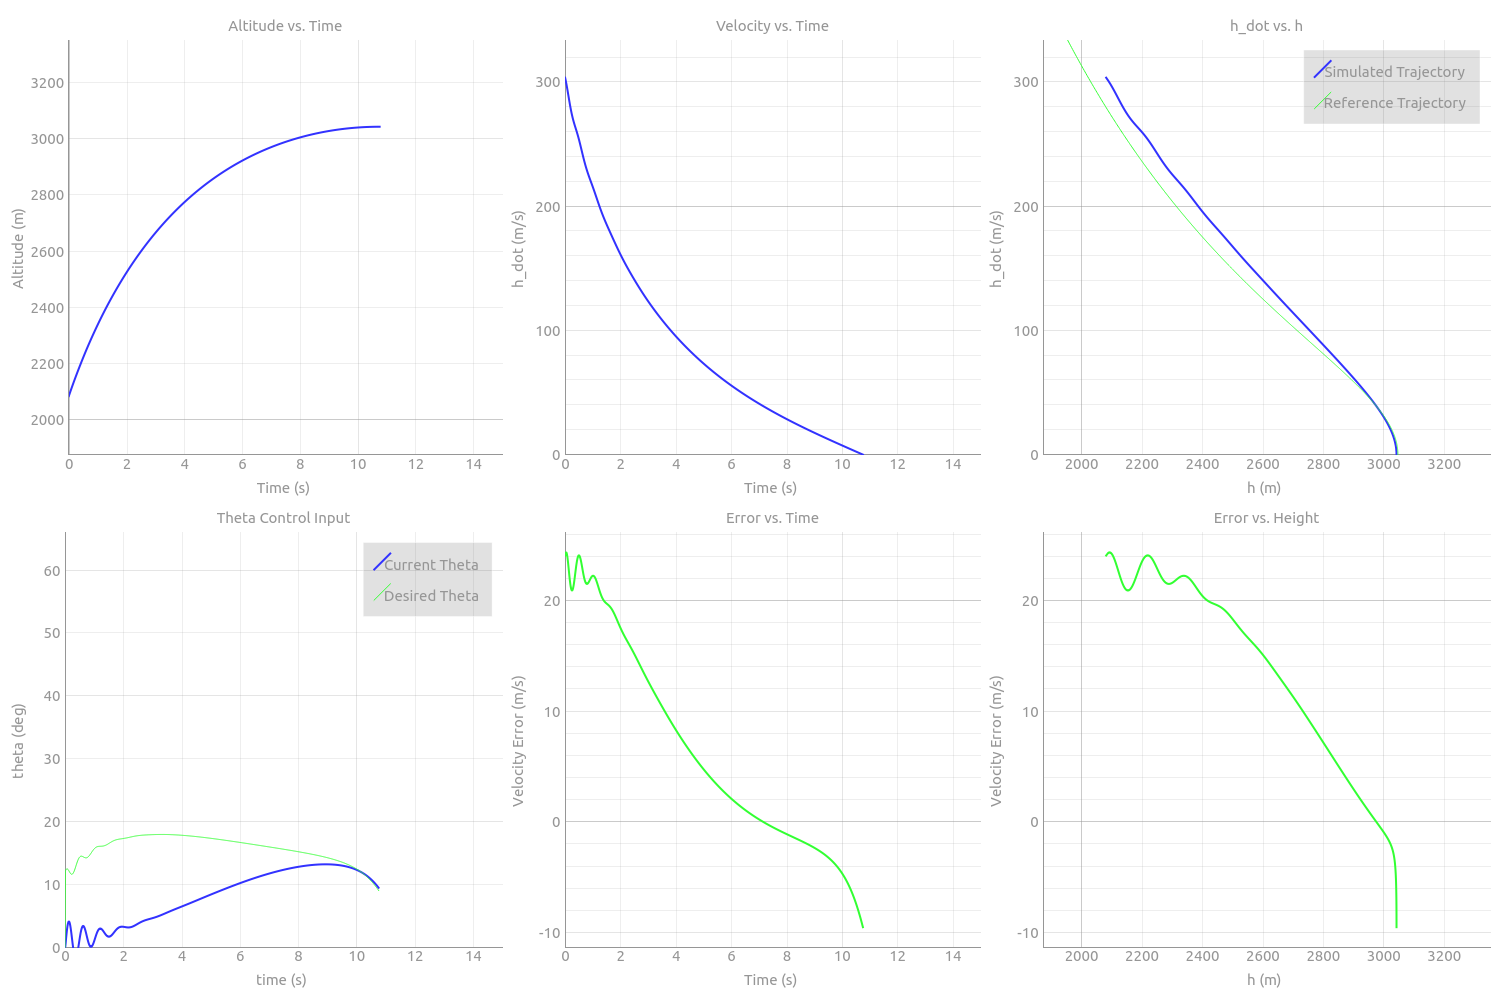
\includegraphics[width=\linewidth]{figures/main.png}
    \caption{The rocket simulation showing the states of interest.}
    \label{fig:main}
  \end{figure}

  More importantly, Figure 2 shows the the estimated and true states. It is worth noting that the simulated barometer had nearly an order of magnitude more noise than what would be expected in implementation on hardware. This was done for the sake of vetting robust estimation. This required some basic low-pass filtering of the derived estimates of states such as $\dot{h}$, $\dot{\theta}$, and $\bar{CD}_0$. The effective time constants of the low-pass filters were chosen based on the speed of the dynamics of the considered state in order to avoid inducing undesirable lag. The estimator functions without this additional filtering, but it was useful for providing better estimate propagations.

  One of the biggest difficulties in the development of the filter was tuning the process noise, $Q$. I created an iterative solver that ran the simulation various times varying a specific element of the $Q$ matrix. The element values increased or decreased in order to minimize the averaged cumulative squared error. This required a lot of computation time, but it effectively found good $Q$ values that were orders of magnitude off from my initial guesses and provided much better performance. See the code for specifics.

  A testament to the effectiveness of the estimator is that the initial drag parameter estimate starts at half the true value and converges to truth in a few iterations. During the rest of flight the estimate isn't perfect, but the reference trajectory generation always uses slightly increased drag, meaning that perfection isn't necessary.

  \begin{figure}
    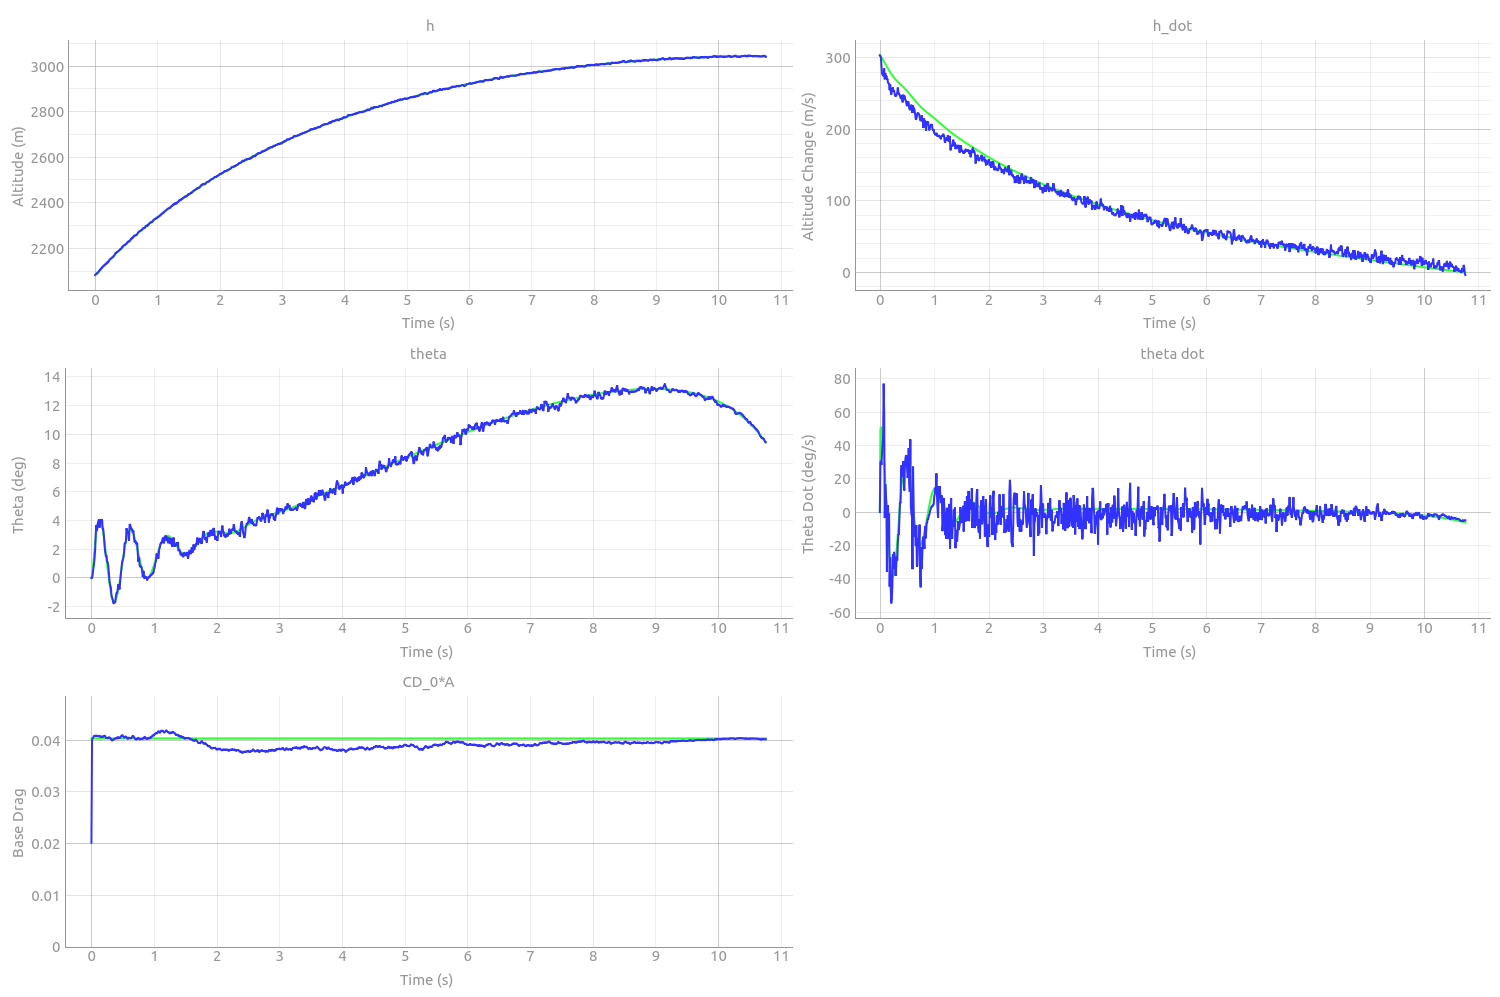
\includegraphics[width=\linewidth]{figures/estimates.png}
    \caption{The state estimates versus truth. Green represents truth and blue represents the estimate.}
    \label{fig:estimates}
  \end{figure}


  \section{Conclusions}
  The work presented in this writeup is merely a first step demonstrating meaningful application of linear system theory to solve this nonlinear problem. As previously stated, control could be improved using feedback linearization. Estimation will likely improve with the use of the Indirect Kalman Filter and realistic noise parameters. Monte Carlo simulation will provide confidence of quality performance in the presense of lots of uncertain parameters.



\end{document}
